\documentclass{standalone}
\usepackage[utf8]{inputenc}
\usepackage{pgfplots}
\DeclareUnicodeCharacter{2212}{−}
\usepgfplotslibrary{groupplots,dateplot}
\usetikzlibrary{patterns,shapes.arrows}
\pgfplotsset{compat=newest}
\begin{document}
% This file was created with tikzplotlib v0.10.1.
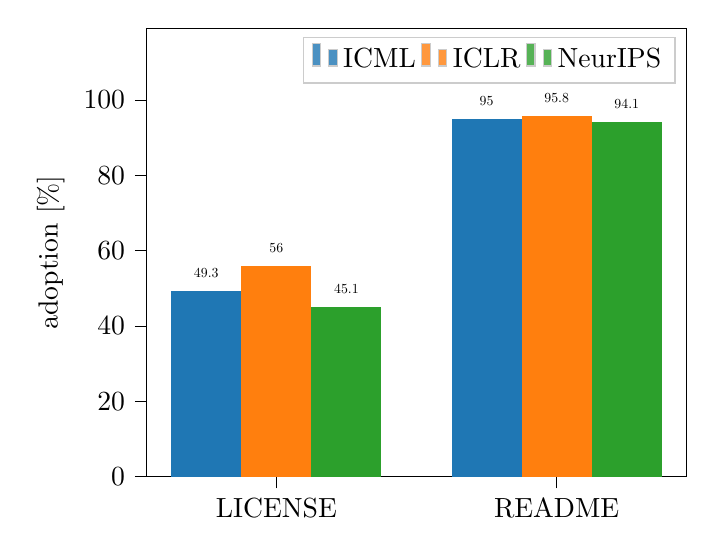
\begin{tikzpicture}

\definecolor{darkgray176}{RGB}{176,176,176}
\definecolor{darkorange25512714}{RGB}{255,127,14}
\definecolor{forestgreen4416044}{RGB}{44,160,44}
\definecolor{lightgray204}{RGB}{204,204,204}
\definecolor{steelblue31119180}{RGB}{31,119,180}

\begin{axis}[
legend cell align={left},
legend columns=3,
legend style={fill opacity=0.8, draw opacity=1, text opacity=1, draw=lightgray204},
tick align=outside,
tick pos=left,
x grid style={darkgray176},
xmin=-0.2125, xmax=1.7125,
xtick style={color=black},
xtick={0.25,1.25},
xticklabels={LICENSE,README},
y grid style={darkgray176},
ylabel={adoption [\%]},
ymin=0, ymax=119,
ytick style={color=black}
]
\draw[draw=none,fill=steelblue31119180] (axis cs:-0.125,0) rectangle (axis cs:0.125,49.3);
\addlegendimage{ybar,ybar legend,draw=none,fill=steelblue31119180}
\addlegendentry{ICML}

\draw[draw=none,fill=steelblue31119180] (axis cs:0.875,0) rectangle (axis cs:1.125,95);
\draw[draw=none,fill=darkorange25512714] (axis cs:0.125,0) rectangle (axis cs:0.375,56);
\addlegendimage{ybar,ybar legend,draw=none,fill=darkorange25512714}
\addlegendentry{ICLR}

\draw[draw=none,fill=darkorange25512714] (axis cs:1.125,0) rectangle (axis cs:1.375,95.8);
\draw[draw=none,fill=forestgreen4416044] (axis cs:0.375,0) rectangle (axis cs:0.625,45.1);
\addlegendimage{ybar,ybar legend,draw=none,fill=forestgreen4416044}
\addlegendentry{NeurIPS}

\draw[draw=none,fill=forestgreen4416044] (axis cs:1.375,0) rectangle (axis cs:1.625,94.1);
\draw (axis cs:0,49.3) ++(0pt,3pt) node[
  scale=0.5,
  anchor=south,
  text=black,
  rotate=0.0
]{49.3};
\draw (axis cs:1,95) ++(0pt,3pt) node[
  scale=0.5,
  anchor=south,
  text=black,
  rotate=0.0
]{95};
\draw (axis cs:0.25,56) ++(0pt,3pt) node[
  scale=0.5,
  anchor=south,
  text=black,
  rotate=0.0
]{56};
\draw (axis cs:1.25,95.8) ++(0pt,3pt) node[
  scale=0.5,
  anchor=south,
  text=black,
  rotate=0.0
]{95.8};
\draw (axis cs:0.5,45.1) ++(0pt,3pt) node[
  scale=0.5,
  anchor=south,
  text=black,
  rotate=0.0
]{45.1};
\draw (axis cs:1.5,94.1) ++(0pt,3pt) node[
  scale=0.5,
  anchor=south,
  text=black,
  rotate=0.0
]{94.1};
\end{axis}

\end{tikzpicture}

\end{document}